\section{Actividad No 09 – SubConsultas} 
		
\begin{enumerate}[1.]
	\item El departamento de Recursos Humanos requiere una consulta que pregunte al usuario por el Apellido del empleado, Luego la consulta deber\'a mostrar los Apellidos y Fecha de Contrataci\'on de todos los empleados del mismo departamento excluyendo o con excepción del empleado el cual ha sido proporcionado su apellido reporte que muestre las direcciones de todos los departamentos.

\begin{itemize}
	\begin{center}
	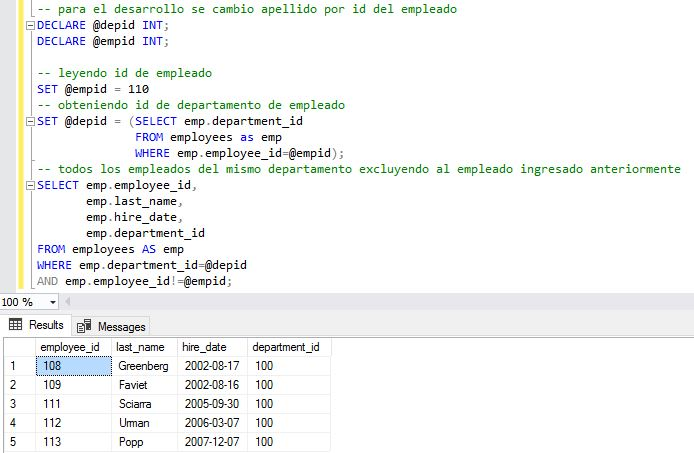
\includegraphics[width=5cm]{./Imagenes/actividad0901} 
	\end{center}
\end{itemize}

	\item Crear un reporte que muestre el No del Empleado, Apellidos y Salarios de todos los empleados que tienen un salario superior al promedio de salarios de todos los empleados. Ordenar los resultados por el Salario de forma ascendente.

\begin{itemize}
	\begin{center}
	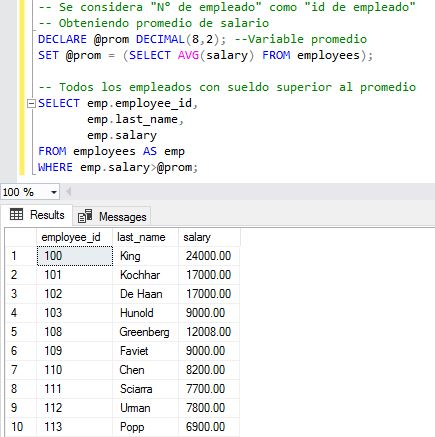
\includegraphics[width=5cm]{./Imagenes/actividad0902} 
	\end{center}
\end{itemize}

	\item Realizar un reporte que muestre el No de Empleado y Apellidos de todos los empleados quienes trabajan

\begin{itemize}
	\begin{center}
	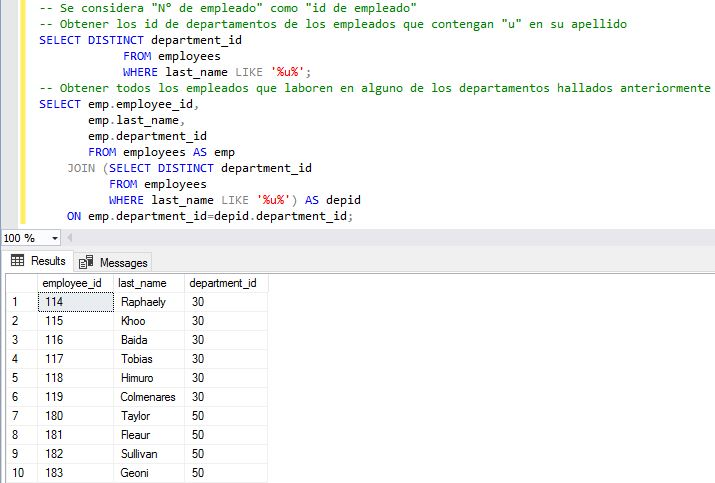
\includegraphics[width=5cm]{./Imagenes/actividad0903} 
	\end{center}
\end{itemize}

en el departamento de cualquier empleado que su apellido contenga la letra ‘u’.
	\item El departamento de Recursos Humanos requiere un reporte que muestre los Apellidos, No de Departamento y Puestos de los empleados cuya locación de departamento es 1700.

\begin{itemize}
	\begin{center}
	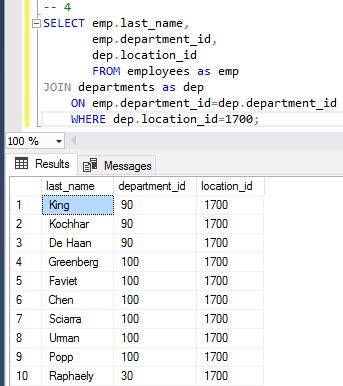
\includegraphics[width=5cm]{./Imagenes/actividad0904} 
	\end{center}
\end{itemize}

	\item Modificar la consulta anterior de forma que el usuario pueda introducir el No de locaci\'on.

\begin{itemize}
	\begin{center}
	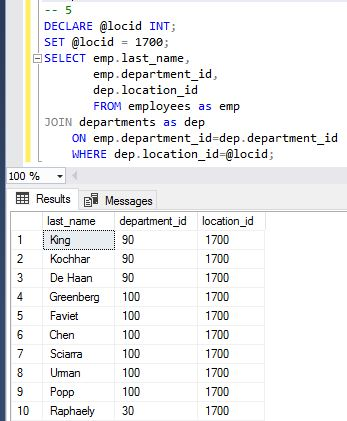
\includegraphics[width=5cm]{./Imagenes/actividad0905} 
	\end{center}
\end{itemize}

	\item Crear un reporte para el departamento de Recursos Humanos que muestre los Apellidos y Salarios de todos los empleados cuyo Administrador apellide ‘King’.

\begin{itemize}
	\begin{center}
	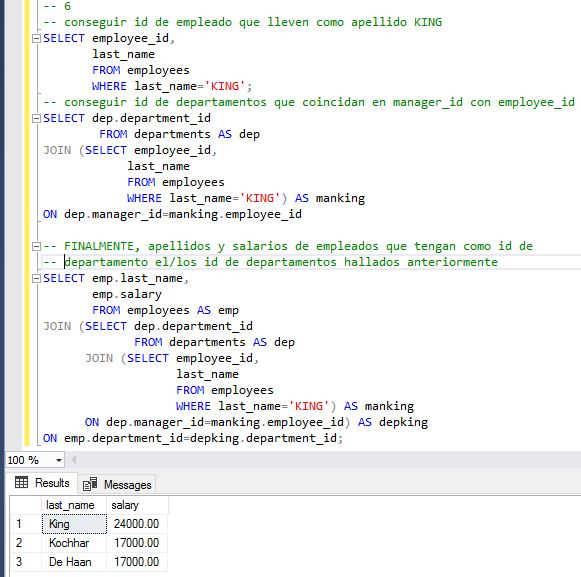
\includegraphics[width=5cm]{./Imagenes/actividad0906} 
	\end{center}
\end{itemize}

	\item Crear un reporte para el departamento de Recursos Humanos que muestre el No de Departamento, Apellidos, Puestos de todos los empleados en el departamento ‘Executive’.

\begin{itemize}
	\begin{center}
	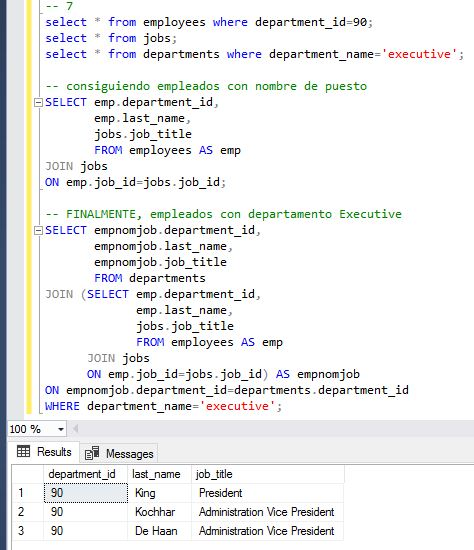
\includegraphics[width=5cm]{./Imagenes/actividad0907} 
	\end{center}
\end{itemize}

	\item Modificar la consulta del ítem 4.3 para que adicionalmente se muestro solo a los empleados que tengan un salario mayor al promedio de todos los salarios de los empleados.
\end{enumerate}
